        
        

\centering
\begin{subfigure}{0.48\linewidth}
\centering
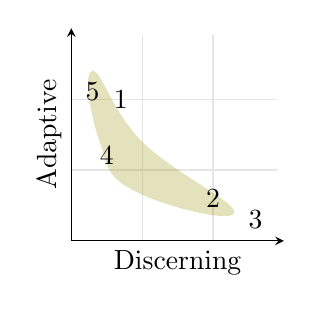
\begin{tikzpicture}[>=stealth,scale=.9,baseline]
    \draw[gray!20] (0,0) grid (2.9,2.9);
    
    \draw[->] (-0,0) -- (3,0);
    \draw[->] (0,-0) -- (0,3);
    
    \node[rotate=90,above] at (0,1.5) {Adaptive};
    \node[below] at (1.5, 0) {Discerning};

    \draw[fill=olive!80, smooth cycle,draw=none,tension=0.8,opacity=0.3] 
      plot coordinates {(0.3, 2.4) (1.0,1.4) (2.3, 0.4) (0.9, 0.7) (0.4, 1.4)};

    \node at (0.7, 2) {\numberedcircle{1}};
    \node at (2, 0.6) {\numberedcircle{2}};
    \node at (2.6, 0.3) {\numberedcircle{3}};
    \node at (0.5, 1.2) {\numberedcircle{4}};
    \node at (0.3, 2.1) {\numberedcircle{5}};

\end{tikzpicture}
\end{subfigure}
\begin{subfigure}{0.48\linewidth}
\centering
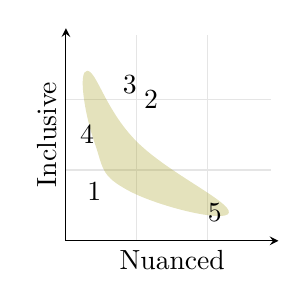
\begin{tikzpicture}[>=stealth,scale=.9,baseline]
    \draw[gray!20] (0,0) grid (2.9,2.9);
    
    \draw[->] (-0,0) -- (3,0);
    \draw[->] (0,-0) -- (0,3);
    
    \node[rotate=90,above] at (0, 1.5) {Inclusive};
    \node[below] at (1.5, 0) {Nuanced};

    \draw[fill=olive!80, smooth cycle,draw=none,tension=0.8,opacity=0.3] 
      plot coordinates {(0.3, 2.4) (1.0,1.4) (2.3, 0.4) (0.9, 0.7) (0.4, 1.4)};



    \node at (0.4, 0.7) {\numberedcircle{1}};
    
    \node at (1.2, 2) {\numberedcircle{2}};  

    \node at (0.9, 2.2) {\numberedcircle{3}};

    \node at (0.3, 1.5) {\numberedcircle{4}};
    \node at (2.1, 0.4) {\numberedcircle{5}};    

\end{tikzpicture}
\end{subfigure}
\caption{Two separate spaces of desiderata; the \textbf{left} represents aspects of \textit{competence}, while the \textbf{right} represents aspects \textit{coverage}.
In each space, there often exists a trade-off between the axes, so that most cultural NLP work falls into the conceptual area that is shaded.}
\label{fig:desiderata}
